\chapter{Conexión local con BD externa} \label{cap:04BDEXt}

Aunque la base de datos de Eunomia permite satisfacer las necesidades ''demo'' de la herramienta, en la mayoría de las ocasiones el objetivo final de la implementación de ATLAS es realizar un estudio o investigación específica sobre una base de datos externa, específica del usuario o la organización que incopora la herramienta de análisis. Por tanto, es de gran interés presentar cómo establecer una conexión adicional entre ATLAS Broadsea y una base de datos personalizada o propia, más allá de la demo que viene inicializada con el contenedor.

La conexión con la base de datos externa se puede realizar de dos formas distintas: 

\begin{enumerate}
    \item La configuración manual, por convención, que utiliza directamente el administrador de la base de datos \ref{cap:04ConfiguracionPgAdmin} y 
    \item La configuración avanzada, por convención, que utiliza los protocolos de seguridad de ATLAS y la webAPI \ref{cap:04ConfigAvanzada}
\end{enumerate}

El manual presenta ambas opciones aunque solo se seguirá en profundidad el protocolo de conexión mediante el administrador de la base de datos, es decir, la configuración manual, ya que es la opción más sencilla y que los propios desarrolladores recomiendan para una implementación rápida \cite{forumAddMSDB}. Por otra parte, por la naturaleza del entorno de instalación al que se enfoca este manual (descrita en \ref{cap:IntroManual}), no es de interés activar el protocolo de seguridad de ATLAS , que debería ser la opción preferente para el despligue de la herramienta en organizaciones donde haya una necesaria diferenciación entre usuarios administradores con privilegios y usuarios sin privilegios. 

%Sin embargo, este caso no aplica puesto que la implementación se realiza para un grupo de investigadores en la que todos tienen los mismos privilegios de acceso.

\section{Configuración manual} \label{cap:04ConfiguracionPgAdmin}

La configuración manual consiste en la conexión con la base de datos externa a través del administrador de la base de datos de Broadsea, en este caso pgAdmin, para realizar consultas sobre la WebAPI de ATLAS que permitan establecer la conexión entre ambas bases de datos. Esta implementación se describe de forma muy completa en la documentación correspondiente al repositorio de github de CDM Configuration \cite{githubCDMConfiguration} y en los foros \cite{forumAddMSDB}\cite{forumBroadQuickStart}.

\subsection{Requisitos previos} \label{cap:04RequisitosPrevios}

- BD en forma CDM
- Ejemplo con synthea: en el mismo servidor,  no hay equema temp, y tampoco vocab porque se va a utilizar el por defecto

\subsection{Deployment}

La conexión con la base de datos es bastante sencilla, basta con configurar los parámetros correspondientes en el esquema \code{webapi} de la base de datos de Broadsea.

\begin{enumerate}
    \item En primer lugar, se debe añadir la nueva fuente en la tabla \code{sources} del esquema \code{webapi}. De este modo se registra la nueva fuente y el string jdbc que apunta hacia ella permitiendo la conexión. Para ello se puede utilizar la siguiente query genérica \cite{githubCDMConfiguration}:

\begin{lstlisting}[language=sql]
INSERT INTO webapi.source (source_id, source_name, source_key, source_connection, source_dialect) 
SELECT nextval('webapi.source_sequence'), 'My Cdm', 'MY_CDM', ' jdbc:postgresql://server:5432/cdm?user={user}&password={password}', 'postgresql';
\end{lstlisting}

    Donde:
    \begin{itemize}
        \item \code{source\_id}: Es el identificador de la fuente. Se asigna por defecto.
        \item \code{source\_name}: Es el nombre personalizado de la fuente.
        \item \code{source\_key}: Es la clave que utilizarán otras tablas para referirse a la fuente.
        \item \code{source\_connection}: Es el string de conexión jdbc, que debe seguir la estructura por defecto que se suigiere en la query. Si la
        \item \code{source\_dialect}: El dialecto que utiliza la base de datos. Por defecto sería postgresql.
    \end{itemize}

    Para la realización de esta implementación de ejemplo se ha seguido el ejemplo de synthea (descrito en \ref{cap:04RequisitosPrevios}), que aplica la siguiente query:

\begin{lstlisting}[language=sql]
INSERT INTO webapi.source (source_id, source_name, source_key, source_connection, source_dialect) 
SELECT nextval('webapi.source_sequence'), 'synthea1k', 'SYNTHEA1K', ' jdbc:postgresql://broadsea-atlasdb:5432/synthea1k?user=postgres&password=mypass', 'postgresql';
\end{lstlisting}

    Esto obtiene como resultado global:

\begin{figure}[H]
    \centering
    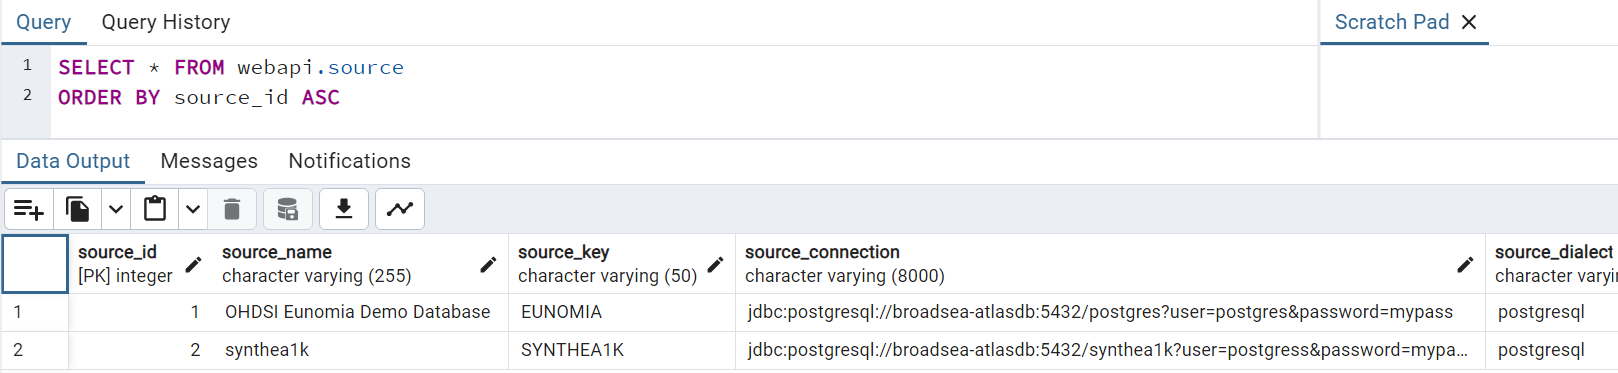
\includegraphics[width=0.90\textwidth]{figures/querySource.png}
    \caption{Captura de pantalla de las fuentes registradas en la tabla \code{sources}.}
    \label{fig:querySource}
\end{figure}
    

    \item En segundo lugar, y por último, se debe registrar cada esquema que utiliza la nueva fuente en la tabla \code{source\_daimon} del esquema \code{webapi}. Para ello se pueden utilizar las siguientes queries genéricas \cite{githubCDMConfiguration}:

\begin{lstlisting}[language=sql]
INSERT INTO webapi.source_daimon (source_daimon_id, source_id, daimon_type, table_qualifier, priority) 
SELECT nextval('webapi.source_daimon_sequence'), source_id, 0, 'cdm', 0
FROM webapi.source
WHERE source_key = 'MY_CDM';

INSERT INTO webapi.source_daimon (source_daimon_id, source_id, daimon_type, table_qualifier, priority) 
SELECT nextval('webapi.source_daimon_sequence'), source_id, 1, 'vocab', 1
FROM webapi.source
WHERE source_key = 'MY_CDM';

INSERT INTO webapi.source_daimon (source_daimon_id, source_id, daimon_type, table_qualifier, priority) 
SELECT nextval('webapi.source_daimon_sequence'), source_id, 2, 'results', 1
FROM webapi.source
WHERE source_key = 'MY_CDM';

INSERT INTO webapi.source_daimon (source_daimon_id, source_id, daimon_type, table_qualifier, priority) 
SELECT nextval('webapi.source_daimon_sequence'), source_id, 5, 'temp', 0
FROM webapi.source
WHERE source_key = 'MY_CDM';
\end{lstlisting}

    Donde:
    \begin{itemize}
        \item \code{source\_daimon\_id}: Es el identificador del daimon. Se asigna por defecto.
        \item \code{source\_id}: Es el identificador de la nueva fuente, según el valor obtenido al registrar la fuente en la tabla \code{sources}.
        \item \code{daimon\_type}: Es el identificador que designa tipo de daimon que se está registrando, es decir, el tipo de esquema. Este identificador puede ser ''0'' para el esquema del \code{cdm}, ''1'' para el \code{vocab}, ''2'' para \code{results} y, opcionalmente, ''5'' para \code{temp}.
        \item \code{table\_qualifier}: Es el nombre concreto del esquema al que se está apuntando.
        \item \code{priority}: Es un valor entero mayor o menor que uno que sirve para distinguir cuál es la fuente prioritaria. Para el vocabulario y results, al menos debe haber un daimon con priority >= 1.  
    \end{itemize}

    Para la realización de esta implementación de ejemplo se ha seguido el ejemplo de synthea (\ref{cap:04RequisitosPrevios}), que aplica las siguiente queries:

\begin{lstlisting}[language=sql]
INSERT INTO webapi.source_daimon (source_daimon_id, source_id, daimon_type, table_qualifier, priority) 
SELECT nextval('webapi.source_daimon_sequence'), source_id, 0, 'synthea', 0
FROM webapi.source
WHERE source_key = 'SYNTHEA1K';

INSERT INTO webapi.source_daimon (source_daimon_id, source_id, daimon_type, table_qualifier, priority) 
SELECT nextval('webapi.source_daimon_sequence'), 2, 1, 'cdm', 1
FROM webapi.source
WHERE source_key = 'SYNTHEA1K';

INSERT INTO webapi.source_daimon (source_daimon_id, source_id, daimon_type, table_qualifier, priority) 
SELECT nextval('webapi.source_daimon_sequence'), 2, 2, 'cdm_results', 0
FROM webapi.source
WHERE source_key = 'SYNTHEA1K';
\end{lstlisting}

    Esto se obtiene como resultado global:

\begin{figure}[H]
    \centering
    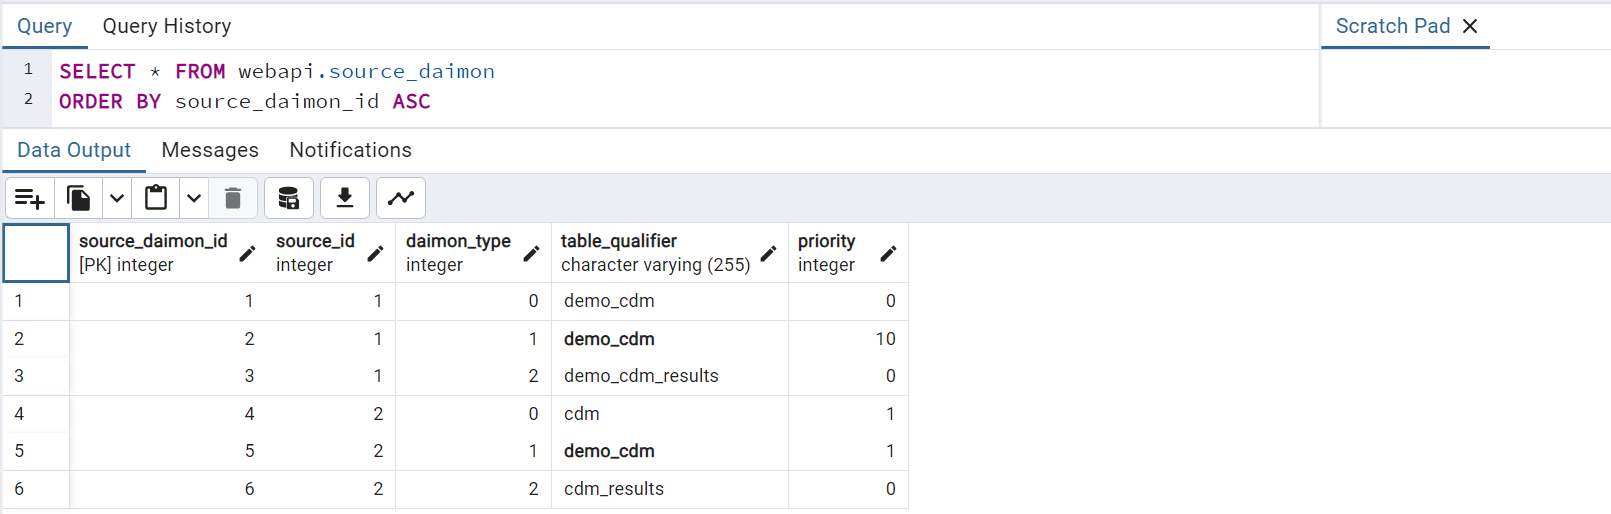
\includegraphics[width=0.90\textwidth]{figures/queryDaimon.png}
    \caption{Captura de pantalla de los daimon registrados en la tabla \code{source\_daimon}.}
    \label{fig:queryDaimon}
\end{figure}

    Observe que si se agrupase por \code{source\_id} hay dos fuentes distintas: (1) la fuente demo que viene preoconfigurada con Broadsea y (2) la fuente que se acaba de registrar.

\end{enumerate}

Así de sencillamente ya estaría registrada la nueva fuente, y establecida la conexión con la misma a través de la webAPI de Broadsea.


\subsection{Comprobación de conexión correcta}

Para comprobar que la conexión con la BD externa se ha realizado correctamente y se ha integrado correctamente con la WebAPI y con ATLAS se puede realizar dos estrategias:

\begin{enumerate}
    \item En primer lugar, acceder a la dirección \code{http://server/WebAPI/source/refresh} en el buscador del navegador y comprobar que aparece como primera fuente la base de datos de Eunomia y los esquemas que utiliza y, como segunda fuente, la base de datos añadida. El resultado debe ser similar al siguiente código:

\begin{lstlisting}[language=sh]
[{"sourceId":1,"sourceName":"OHDSI Eunomia Demo Database","sourceDialect":"postgresql","sourceKey":"EUNOMIA","daimons":[{"sourceDaimonId":1,"daimonType":"CDM","tableQualifier":"demo_cdm","priority":0},{"sourceDaimonId":3,"daimonType":"Results","tableQualifier":"demo_cdm_results","priority":0},{"sourceDaimonId":2,"daimonType":"Vocabulary","tableQualifier":"omop_vocab","priority":10}]},

{"sourceId":2,"sourceName":"synthea1k","sourceDialect":"postgresql","sourceKey":"SYNTHEA1K","daimons":[{"sourceDaimonId":4,"daimonType":"CDM","tableQualifier":"cdm\n","priority":1},{"sourceDaimonId":5,"daimonType":"Vocabulary","tableQualifier":"omop_vocab","priority":1},{"sourceDaimonId":6,"daimonType":"Results","tableQualifier":"cdm_results","priority":0}]}]
\end{lstlisting}

    \item En segundo lugar, comprobar a través de la interfaz gráfica de ATLAS que aparece la nueva fuente, a través del menú deplegable del apartado \code{Data sources} o en el apartado \code{Configuration} de la herramienta.

\begin{figure}[H]
    \centering
    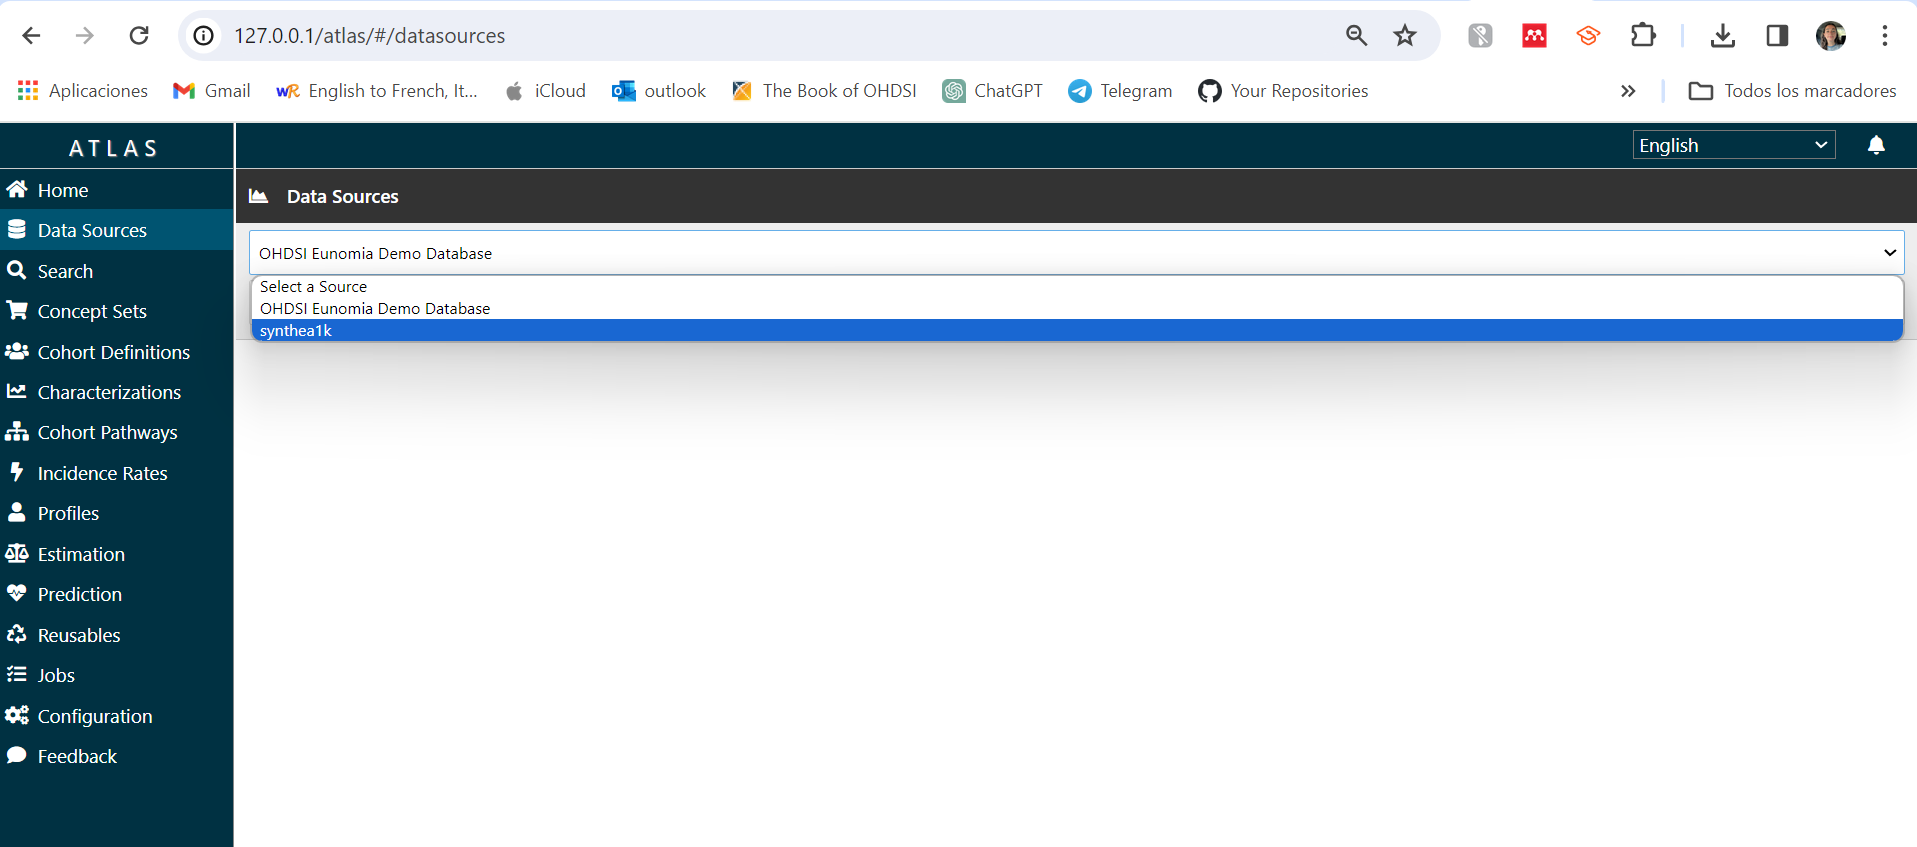
\includegraphics[width=0.90\textwidth]{figures/showDataSources.png}
    \caption{Captura de pantalla del menu \code{Data sources} de ATLAS Broadsea}
    \label{fig:showDataSources}
\end{figure}

\begin{figure}[H]
    \centering
    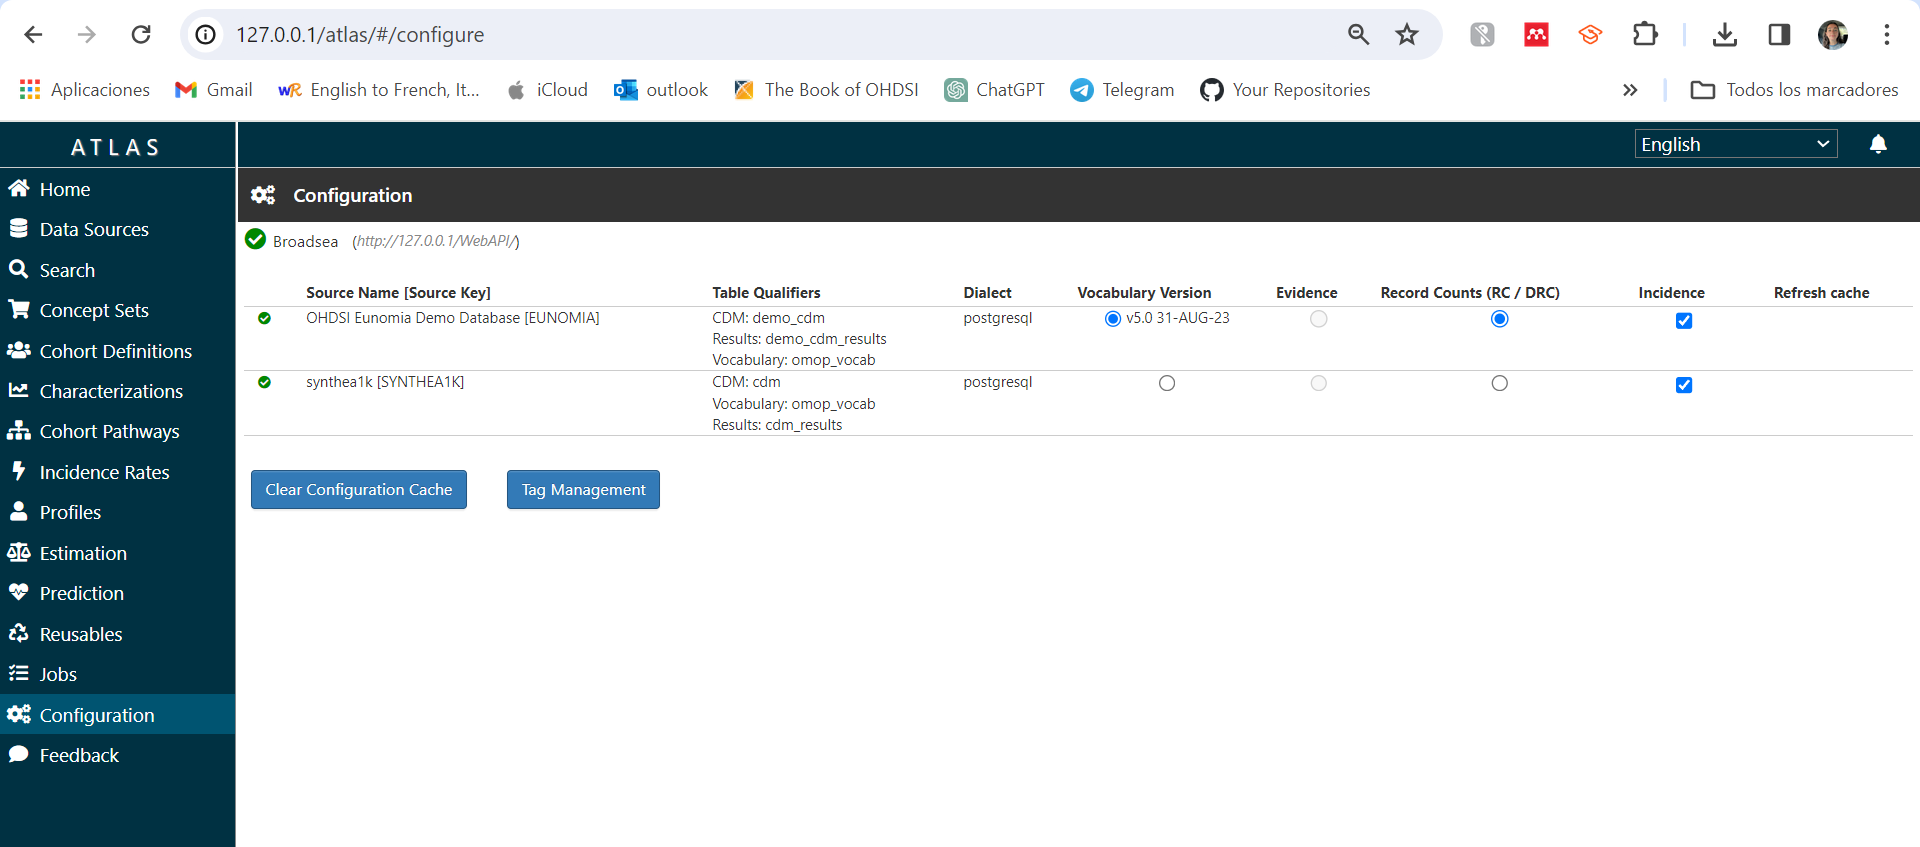
\includegraphics[width=0.90\textwidth]{figures/showConfiguration.png}
    \caption{Captura de pantalla del menu \code{Configuration} de ATLAS Broadsea}
    \label{fig:showConfiguration}
\end{figure}
\end{enumerate}


\subsection{Solución de posibles problemas}

- Faltan esquemas no aparece
- Valores mla introducidos

\section{Otras configuraciones avanzadas} \label{cap:04ConfigAvanzada}

\subsection{Configurar la seguridad de ATLAS}

Otra forma de establecer conexiones con bases de datos externas es activando el protocolo de seguridad de ATLAS y de la WebAPI. Esta configuración posibilita la adición de fuentes a través de la interfaz gráfica de ATLAS, pues crea en el menú \code{Configuration} un nuevo boton para añadir fuentes intuitivamente. 

\begin{figure}[H]
    \centering
    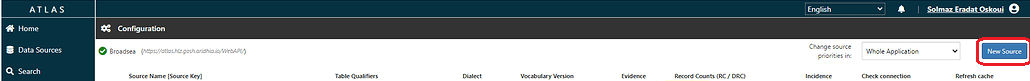
\includegraphics[width=0.90\textwidth]{figures/capNewSource.png}
    \caption{Imagen extraída de \cite{forumAddMSDB} donde aparece el botón para añadir fuentes desde la interfaz gráfica de ATLAS}
    \label{fig:capNewSource}
\end{figure}

No obstante, esta forma tan aparentemente sencilla de conexión, verdaderamente se establece a través de protocolos complejos y configuraciones avanzadas de ATLAS y la WebAPI que resultan en grandes cantidades de problemas y errores. De hecho, en varias ocasiones los propios desarrolladores a través de los foros recomiendan su uso solo cuando sea extrictamente necesario \cite{forumAddMSDB}\cite{forumAddSecurityAtlas}.

Si bien la configuración es compleja, aporta, además de la facilidad de adición de fuentes mediante el botón en ATLAS, la posibilidad de distinguir entre distintos usuarios y roles con distintos permisos y privilegios, lo cual puede ser de gran interés en ciertos entornos u organizaciones.  La configuración de la seguridad de ATLAS empieza por la configuración de la seguridad de la WebAPI y ambas están descritas detalladamente en los correspondientes repositorios de Github \cite{githubWASecurity}\cite{githubATSecurity}. También hay un foro de gran interés en el que se describen aspectos de utilidad sobre la configuración de la seguridad en una organización \cite{forumAddSecurityAtlas}.

\subsection{Descargar otras BD}
- synthea
- synpuf